\chapter{Implementation}
This chapter describes the implementation of GeoDude and some of the considerations behind the choices as well as the functionality.

\section{GPS module}
The knowledge about pin assignments for the GPS module, RGM-2000, comes from the website: \url{http://www.tobias-schlegel.de/?page_id=51&lang=en}.\\
The communication settings were found in the User Manual (RGM-2000\_user\_manual.pdf which can be found in appendix). This is the same for all GPS modules using that standard. The settings are as follows:
\begin{table}[H]
    \begin{tabular}{|ll|}
    \hline
    Baud rate    & : 4800 \\ \hline
    Data bit     & : 8    \\ \hline
    Parity       & : None \\ \hline
    Stop bit     & : 1    \\ \hline
    Flow control & : None \\ \hline
    \end{tabular}
    \caption{UART setup in NMEA-0183 standard}
\end{table}
To understand the format output from the GPS module, NMEA-0183, we consulted the wikipedia site as well as observing on Tx in RealTerm (terminal software). The raw NMEA-0183 string looks like this:
\begin{verbatim}
$GPGGA,092750.000,5321.6802,N,00630.3372,W,1,8,1.03,61.7,M,55.2,M,,*76
\end{verbatim}
To display this data in an understandable way, we have to cut the string up and "send" it. This is done in a smart way in C code:
\begin{lstlisting}{language=C}
while((GPSD->gpsstring[j]) != COMMA) // Read lateral string until Comma
{
	GPSD->latString[k] = (GPSD ->gpsstring[j]);
	if(k == 3)
	{
		k++;
		GPSD->latString[k] = '*';   
		// the degree symbol doesnt exist in ascii. 
		// Asterisk is a placeholder
	}
	j++;
	k++;
}
\end{lstlisting}
By running through the GPS string until a comma is found, we can catch every snippet. The snippets are put into string found in the GPSDATA struct. The struct can be found in gps.h (in appendix gps.h.pdf).

\section{Screen}
The screen is a nokia 3310 display controlled by a PCD8544. The PCD8544 has a SPI interface along with three control pins. These pins are: Chip enable, reset and data/command pin.\\
The data/command pin is used to tell the display whether a command or data has been transmitted. Below a figure from the datasheet is displayed, showing how a transmission should be done.

\begin{figure}[H]
\centering
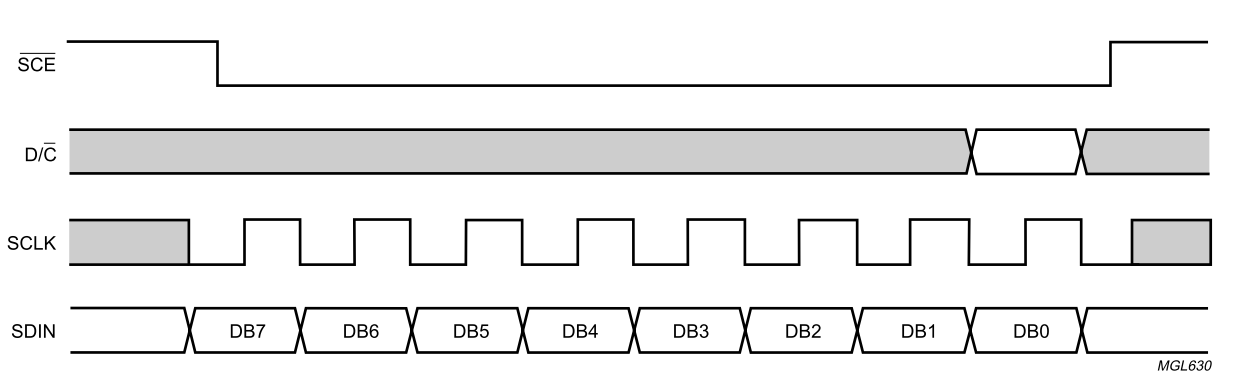
\includegraphics[width=.8\textwidth]{billeder/Display_protocol}
\caption{PCD8544 serial bus protocol one byte transmission}
\end{figure}

Commands to the display is used for setup purposes such as contrast, cursor position, ram addressing etc. Data to the display is used to set the pixels to either on or off. The display is divided into "banks" where a bank consists of 8 pixels(horizontal). It has 6 banks in height and 84 banks in width.\\
Using horizontal addressing of these RAM banks allows for easy writing of chars. Making this neat little trick we can use chars as input to this function. This function is then used in our \texttt{LCD\_WriteString}  function to get a simple "printf"-like functionality.
\begin{lstlisting}{language=C}
void LCD_WriteChar(unsigned char ch)
{
	int i;
	for (i=0; i < ch_width ; i++ )
	{
		LCD_Write_data( pgm_read_byte( &(Font [(ch-32)*5 + i] )));	
	}
	LCD_Write_data(0x00);			
}
\end{lstlisting}
The "Font" array is a large array that, along with the "Arrow" array (which holds data for the 8 direction arrows), have been placed in the \texttt{PROGMEM} area. At first it wasn't placed here but when we incorporated FreeRTOS to the project we ran out of space. Placing it in \texttt{PROGMEM} made enough space to support FreeRTOS.\\
Below is shown a little part of the Font array:
\begin{lstlisting}{language=C}
static const unsigned char Font[] PROGMEM =
{
	0x00, 0x00, 0x00, 0x00, 0x00,   // sp 
	0x00, 0x00, 0x2f, 0x00, 0x00,    // ! 
	0x00, 0x07, 0x00, 0x07, 0x00,   // "  
	0x14, 0x7f, 0x14, 0x7f, 0x14,   // #  
	0x24, 0x2a, 0x7f, 0x2a, 0x12,   // $  
	....  
};
\end{lstlisting}

The first spot in the array is the 32nd place in the ascii table, therefore we substract 32 from the ch input in the LCD\_WriteChar function when accessing the array. We also multiply by 5 since each char is 5 pixels wide. We found the Font array via google search.

\section{Magnetometer}
The magnetometer is a HMC6352 and is interfaced using i$^2$c. It is a fully implemented compass with everything handled. It has a register that  the setup is written to. We set the magnetometer to 10Hz measurement rate, periodic set/reset on, which is factory default, but we wanted to make sure that we know how and what it is set to.\\
The Magnetometer runs at 100kbps. To get the ATmega32 i$^2$c to run at this rate we setup the TWSR and TWBR register.\\
$\frac{8MHz}{16+2*TWBR}=100kbps, TWBR = 32$ which is exactly 100kHz\\
In the datasheet a table is shown were all responses are described.

\begin{table}[H]
\centering
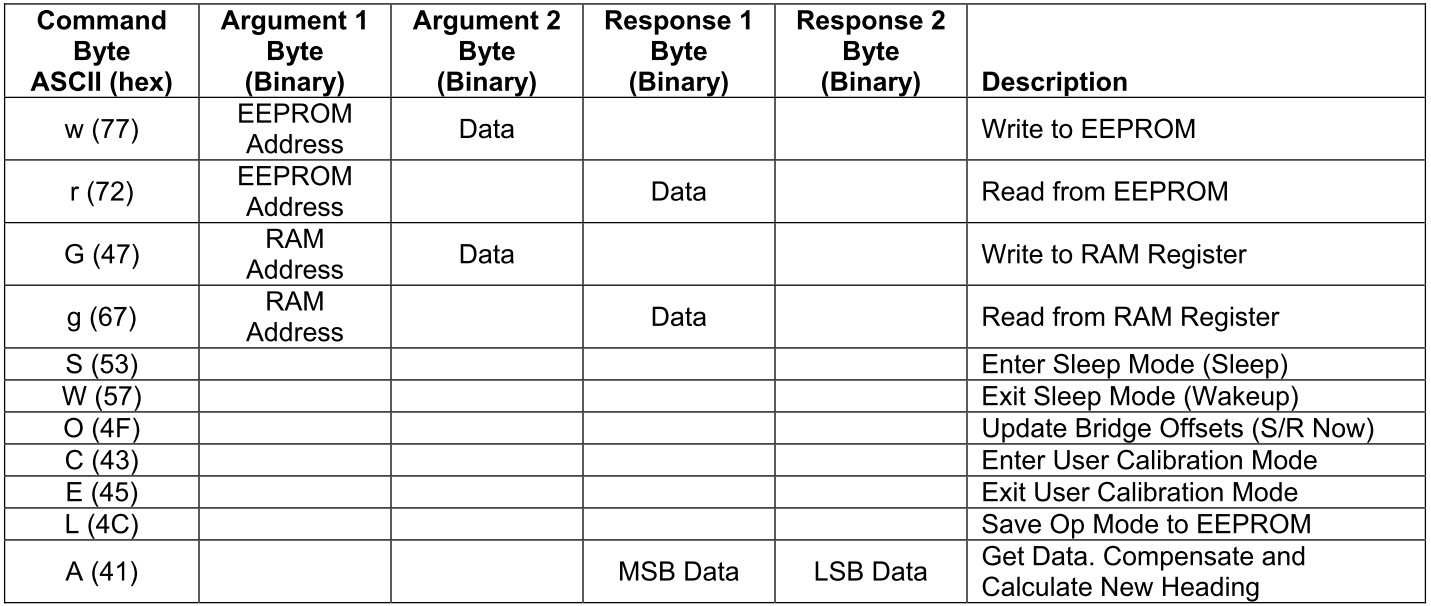
\includegraphics[width=.9\textwidth]{billeder/HMC6352_responses}
\caption{HMC6362 Request and response table}
\end{table}

This table was used to identify a transmit/receive sequence. Below is shown an example from the datasheet illustrating a read from a RAM register.

\begin{figure}[H]
\centering
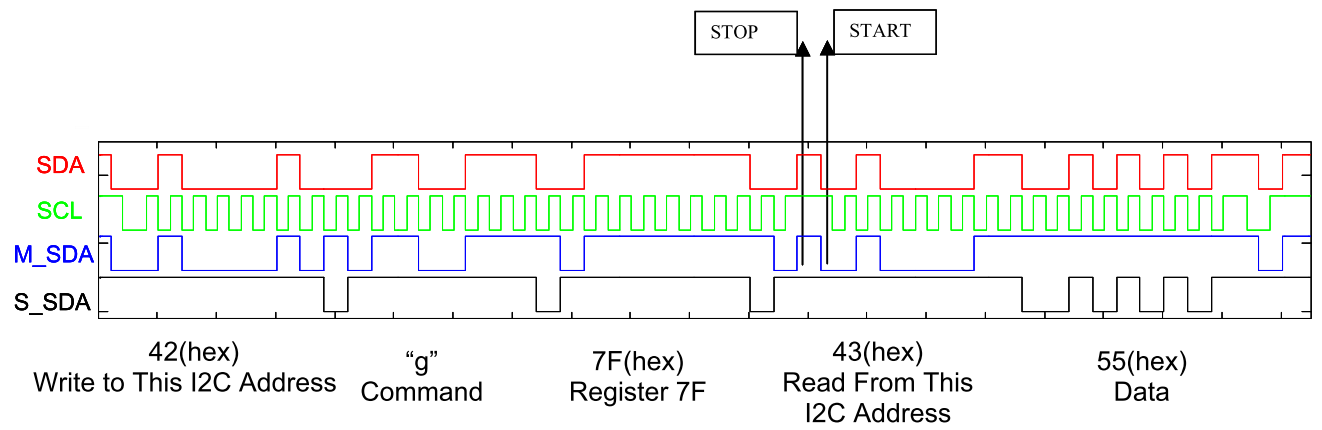
\includegraphics[width=.8\textwidth]{billeder/HMC6352_example}
\caption{HMC6352 write + read sequence}
\end{figure}

A transfer/receive sequence is, as usual in i$^2$c, initiated by a "start" from the master by first pulling SDA low and then the SCL. Hereafter the master sends the address indicating a write and then the commands to the slave. When the commands have been sent the transmission is stopped, and then started again shortly after with the read address and the slave responds with the data.\\
The heading value from the magnetometer is returned in 10th of degrees, therefore ranging from 0 to 3599. This value is then converted into eights of a circle for the screen API to use.\\
There are no pull-up resistors on the HMC6352, these are added externally (see Demo Board).\\

\section{Software structure}
The software implemented in this project is described by the UML diagram in the figure below.\\
The system is described via. UML even though it is made in C it offers a nice overview of all headers, variables and function calls.\\

\begin{figure}[H]
\centering
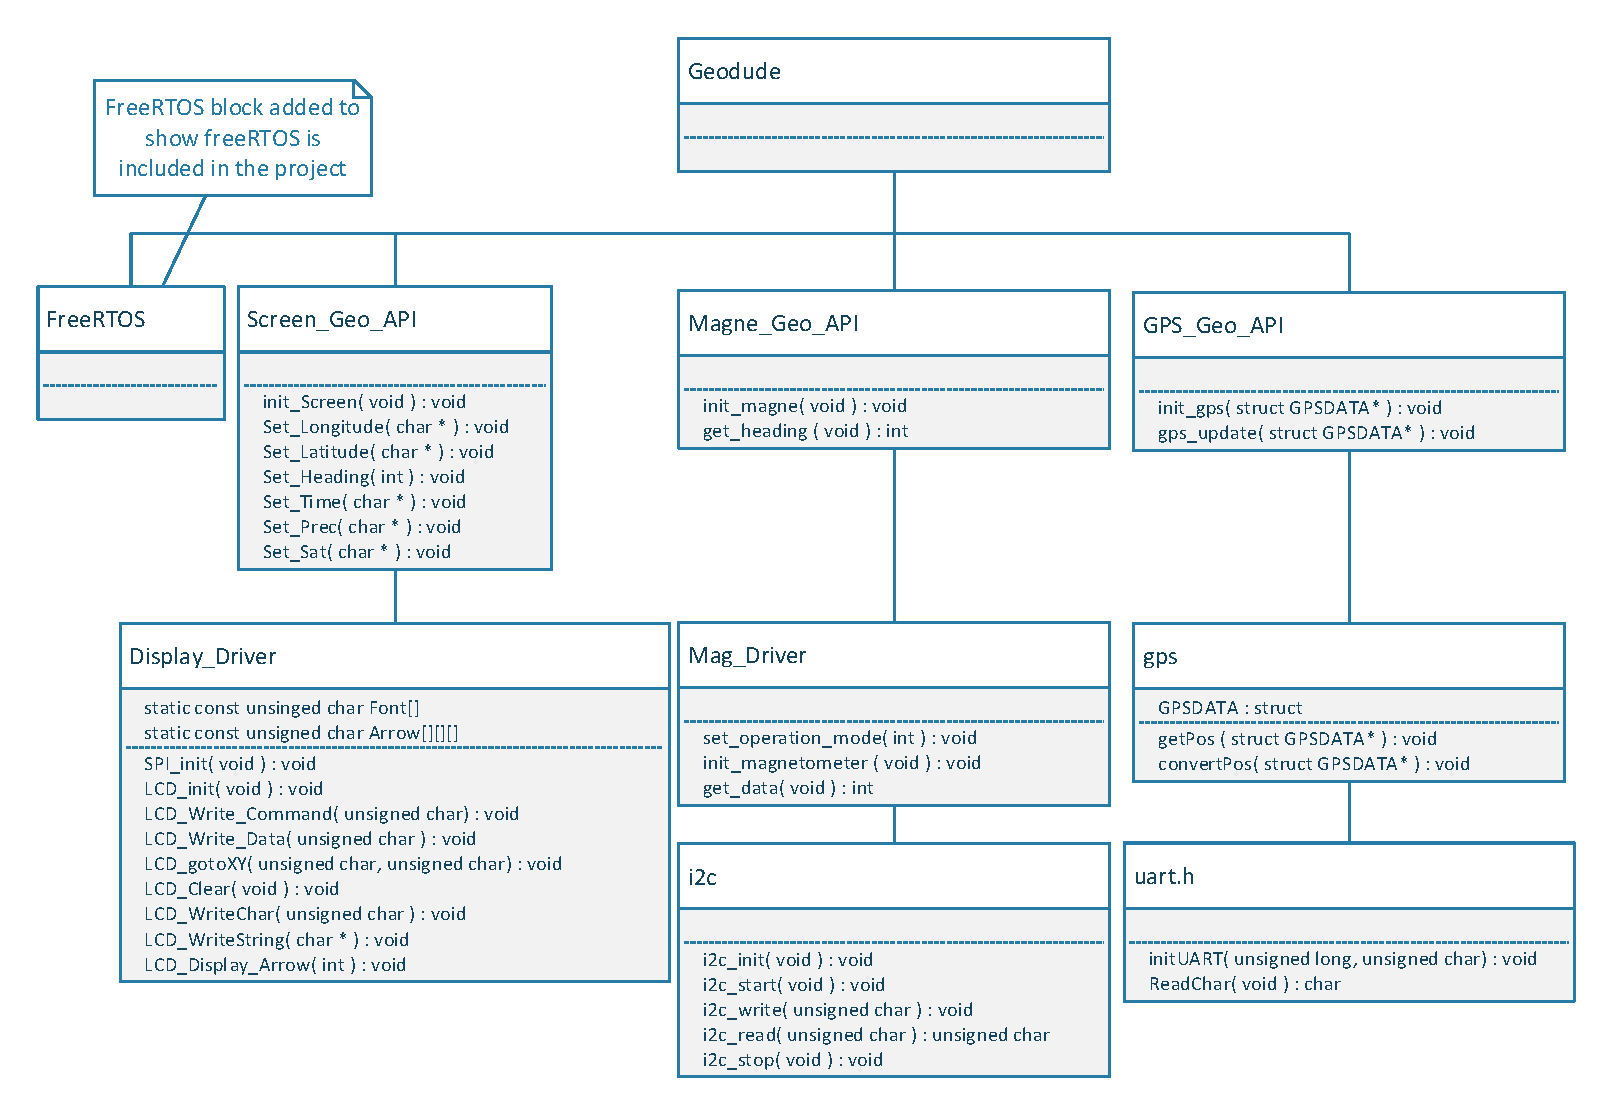
\includegraphics[width=1\textwidth]{billeder/geodude_UML}
\caption{Geodude UML diagram}
\end{figure}

\begin{wrapfigure}{r}{5cm}
\vspace{-30pt}
\begin{center}
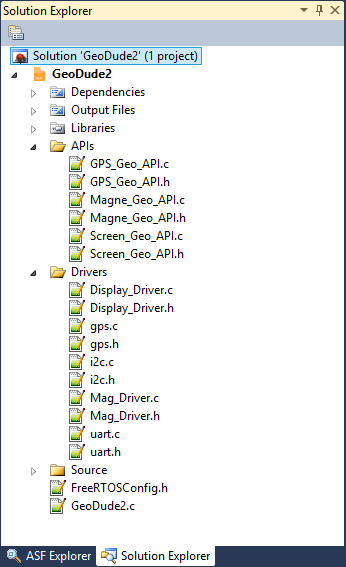
\includegraphics[width=4cm]{billeder/folder_structure}
\end{center}
\vspace{-20pt}
\caption{Geodude software folder structure}
\vspace{-20pt}
\label{fig:fold_structure}
\end{wrapfigure}
The system is implemented by making API's specific to our application by using generic drivers. This makes the system easy to port to another platform if this is insufficient at some point in the implementation.\\
We also chose to implement FreeRTOS onto our system. Our thoughts behind this choice was to make it easy to scale the project and implement more tasks. As mentioned in the introduction the stage of the project in this course is not the intended end project. Therefore it is important to keep in mind that several other tasks might be added. If this is not possible because it was implemented using one big superloop in main the initial work would not be worth that much.\\%
The two drivers i2c and uart have been acquired from the course ITAMS.\\
The project folder structure, as seen on figure \ref{fig:fold_structure}, is divided into "Drivers", "API's" and "Source". This makes for an easy overview when working on the project.\\

\subsection{FreeRTOS}
%Noget med de settings der er valgt med opsætning af heap, ticks til tasks, og hvilke tasks der er lavet og hvorfor
We started with the FreeRTOS project provided by the ITAMS course. We corrected the settings according to our system by setting the clock to 8 MHz.  We made 4 tasks for the scheduler:
\begin{lstlisting}{language=C}
void vUpdateScreen( void *pvParameters )
{
	//Updates screen with GPS data if is has been updated.
	//Updates heading
}
void vUpdateGPS( void *pvParameters )
{
	//Updates GPSdata
}
void vUpdateHeading( void *pvParameters )
{
	//Updates Heading
}
void vBootLoad( void *pvParameters )
{
	// Enters Bootloader section if button is pressed
}
\end{lstlisting}
We use the vTaskDelayUntil function to tell when to enter the different tasks. The time setup is defined like this:
\begin{lstlisting}{language=C}
#define UPDATEGPSTIME 150
#define UPDATESCREENTIME 300
#define BOOTLOADTIME 500
#define UPDATEHEADINGTIME 200
\end{lstlisting}



\subsection{Bootloader}
%Noget med at vi er opmærksomme på størrelsen af programmet og hvor bootloaderen ligger
%også noget med internal oscilator og uart? eller er det ligegyldigt?
%noget med at bootloader fordi vi laver et demoboard?
%Hvorfor (Noget med demoboard og portation til virkeligheden.
To program the system we started out by using the STK500 programmer. When we moved the ATmega32 to our demoboard, described in section~ \ref{sec:demob}, we needed a better way to program the chip. We chose to implement a bootloader onto our system for easy programming and updating of the firmware. The bootloader was provided by the ITAMS course.\\
The internal clock in our system is 8 MHz so we have to select a proper baud rate for communication for the programming software on the PC to work. From uart.c in the bootloader:
\begin{lstlisting}{language=C}
#define XTAL 8000000  

__attribute__ ((section (".bootloader"))) // bootloader section
void InitUART()
{...
	// Write upper part of UBRR
  UBRRH = ((XTAL/16)/38400 - 1) >> 8;
  // Write lower part of UBRR
  UBRRL = ((XTAL/16)/38400 - 1);
}
\end{lstlisting}
We found that 38400 baud worked really well with our 8 MHz internal clock.\\
The software used for programming is AvrOspII\footnote{AvrOspII has been acquired through code.google.com because the original website is not functional}. AvrOspII was chosen because of the ability to easily change baud rate and com port.\\
When programming, we compile in AVR studio 6 and enter the hex file in AvrOspII.\\
The bootloader can also be used in the final product to update the firmware making it a solid choice to implement it in our project.\\

\section{Demo board}
\label{sec:demob}
This section briefly describes the demo board developed to make the application portable.\\
Below is shown the connections made on the breadboard\footnote{None of the values are noted since they are not relevant with regards to the course.} for the project. This was made to make the application portable so we were able to go outside and test the satellite connection etc.\\

\begin{figure}[H]
\centering
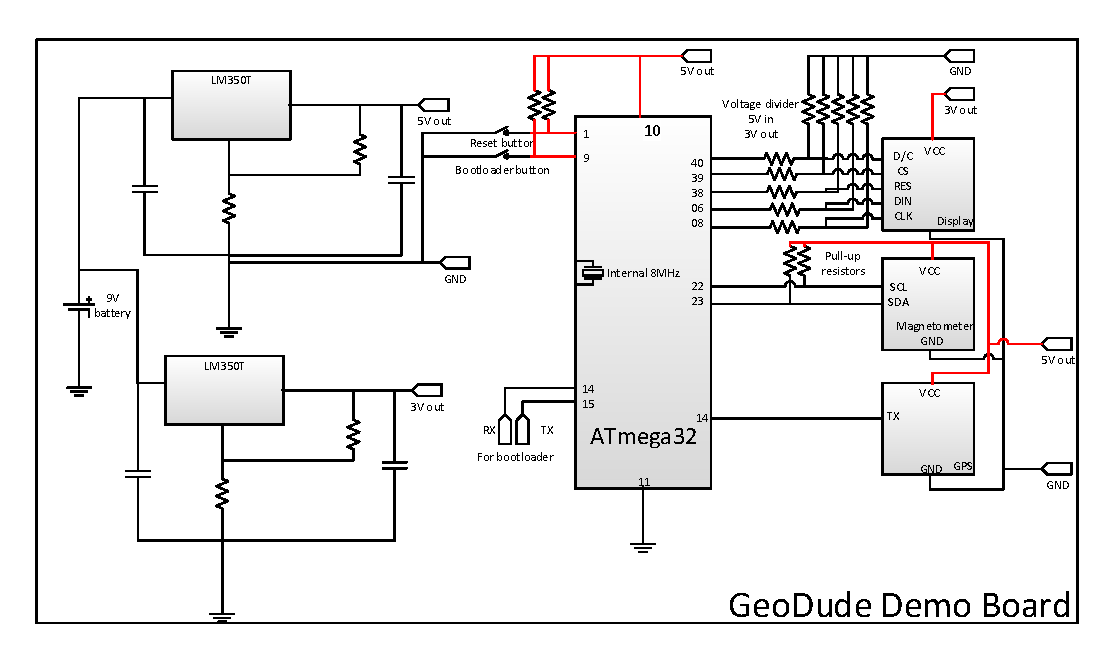
\includegraphics[width=1\textwidth]{billeder/GeodudeDemoBoard}
\end{figure}

The circuit is powered by a 9V battery which is regulated to 5V to supply the ATmega32, the GPS module and the magnetometer and 3V to supply the screen.